\documentclass[12pt]{article}

\usepackage[utf8]{inputenc}
\usepackage[russian]{babel}
\usepackage{amsmath}
\usepackage{setspace}

\usepackage{caption}
\usepackage{subcaption}
\usepackage{float}
\usepackage{graphicx}
\graphicspath{ {./images/} }

\usepackage{geometry}
 \geometry{
 a4paper,
 left=20mm,
 right=20mm,
 top=20mm,
 bot=20mm,
 }

\begin{document}

\begin{titlepage}
\begin{center}
    {\small НАЦИОНАЛЬНЫЙ ИССЛЕДОВАТЕЛЬСКИЙ УНИВЕРСИТЕТ ИТМО} \\
    {\small Факультет систем управления и робототехники} \\
    \vspace*{10\baselineskip}
    {\LARGEЭлектроника и схемотехника} \\
    \ \\
    \begin{spacing}{1.5}
    {\large Лабораторная работа №4 \\
    Исследование характеристик тиристора и управляемых схем на тиристорах} \\
    \end{spacing} \\
    \ \\
    Вариант 2 \\
    \vspace*{10\baselineskip}
    \hfill {Выполнили студенты:} \\
    \hfill {Кирбаба Д.Д. R3338} \\
    \hfill {Курчавый В.В. R3338} \\
    \ \\
    \hfill {Преподаватель:} \\
    \hfill {Николаев Н.А.} \\
    \mbox{}
    \vfill {г. Санкт-Петербург\\2023}
\end{center}
\end{titlepage}

\section*{Цель работы}
Углубленное изучение тиристора, исследование схемы управляемого выпрямителя и тиристорного регулятора мощности.

\section*{Ход работы}
Вариант 2.\\
Тиристор: EC103M1. \\
Характеристики:
\begin{itemize}
    \item $I_{bo} = 20 \ A$ - ток переключения;
    \item $V_{bo} = 600 \ V$ - напряжение переключения;
    \item $V_{o} = 1.7 \ V$ - напряжение открытого состояния;
    \item $I_{{off}_{sl}} = 1 \ \mu A$ - утечка тока в выключенном состоянии;
    \item $I_{{on}_{sl}} = 0.8 \ A$ - учечка тока во включенном состоянии;
    \item $V_{pi} = 1.2 \ V$ - допустимое обратное напряжение;
    \item $V_{gt} = 0.8 \ V$ - напряжение срабатывания затвора;
    \item $I_{gt} = 12 \ \mu A$ - ток срабатывания затвора.
\end{itemize}

\subsubsection*{Исследование работы управляемого выпрямителя}

\begin{figure}[H]
    \centering
    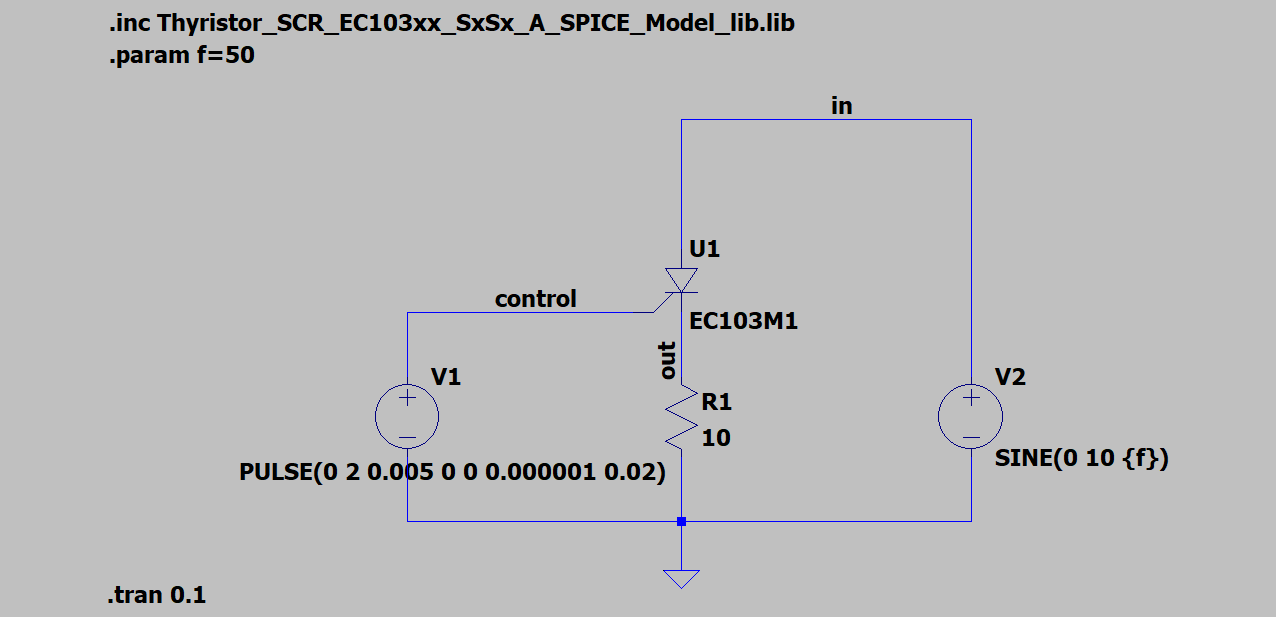
\includegraphics[width=0.7\textwidth]{1_scheme.png}
    \caption{Схема моделирования однополупериодного управляемого выпрямителя.}
    \label{fig:1_scheme}
\end{figure}

Для управления включением тиристора необходимо выполнить два условия: напряжение на аноде тиристора должно быть положительным (но не превышающим напряжения переключения $V_{bo}$) и к управляющему электроду должно быть приложено положительного напряжение соответствующее напряжению отпирания $V_{gt}$. \\
\ \\
Источник входного напряжения будет генерировать синусоидальный сигнал с частотой $f_{in} = 50 \ Hz$, амплитудой $V_{{in}_{amp}} = 10 \ V$. \\
\ \\
Амплитуду управляющего сигнала установим равной $V_{control} = 2 \ V$. \\
Угол включения сделаем равным $\alpha = 90^\circ$. \\
\ \\
Снимем осциллограммы входного, выходного и управляющего сигналов:
\begin{figure}[H]
    \centering
    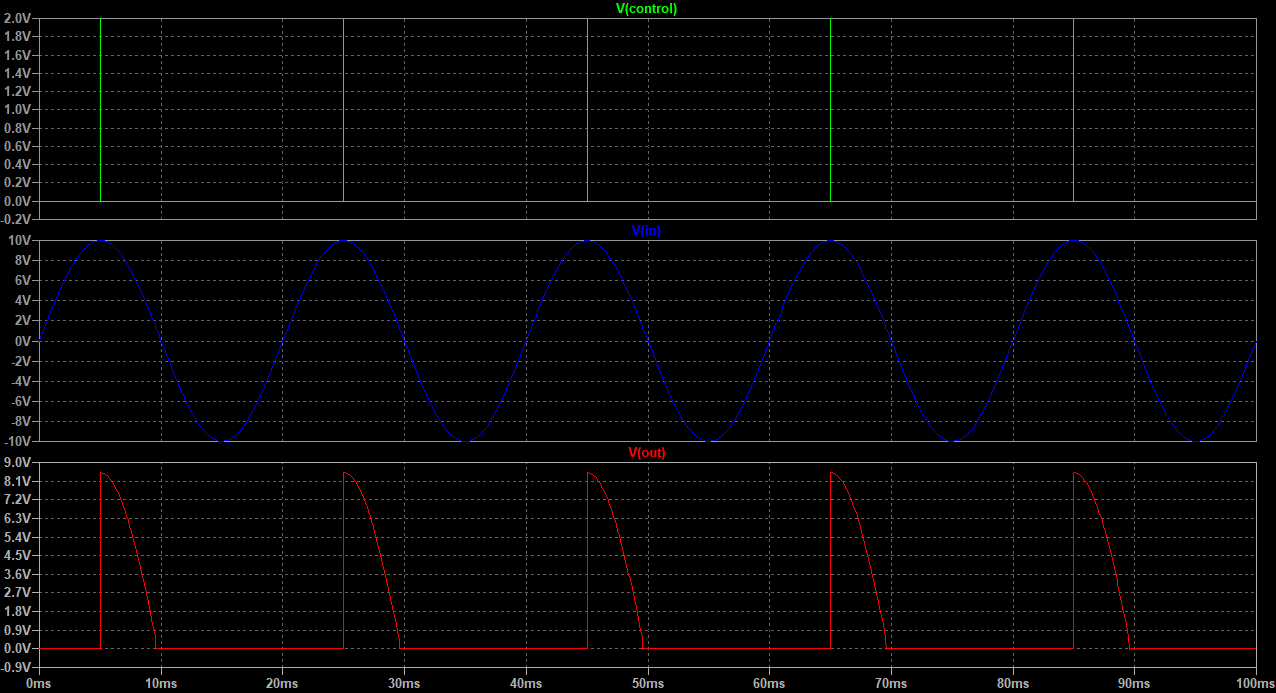
\includegraphics[width=\textwidth]{1_out_in_conrtrol_v.png}
    \caption{Осциллограммы входного, выходного и управляющего сигналов.}
    \label{fig:1_out_in_control_v}
\end{figure}

Рассчитаем среднее значение напряжения на нагрузке:
\[
    V_{load_{mean}} = \frac{1}{2\pi} \int_{\alpha}^{\pi} V_{in} \,d(\omega t) = \frac{V_{{in}_{amp}}}{2\pi}(1+\cos{\alpha}) = 1.59 \ V.
\]

\begin{figure}[H]
    \centering
    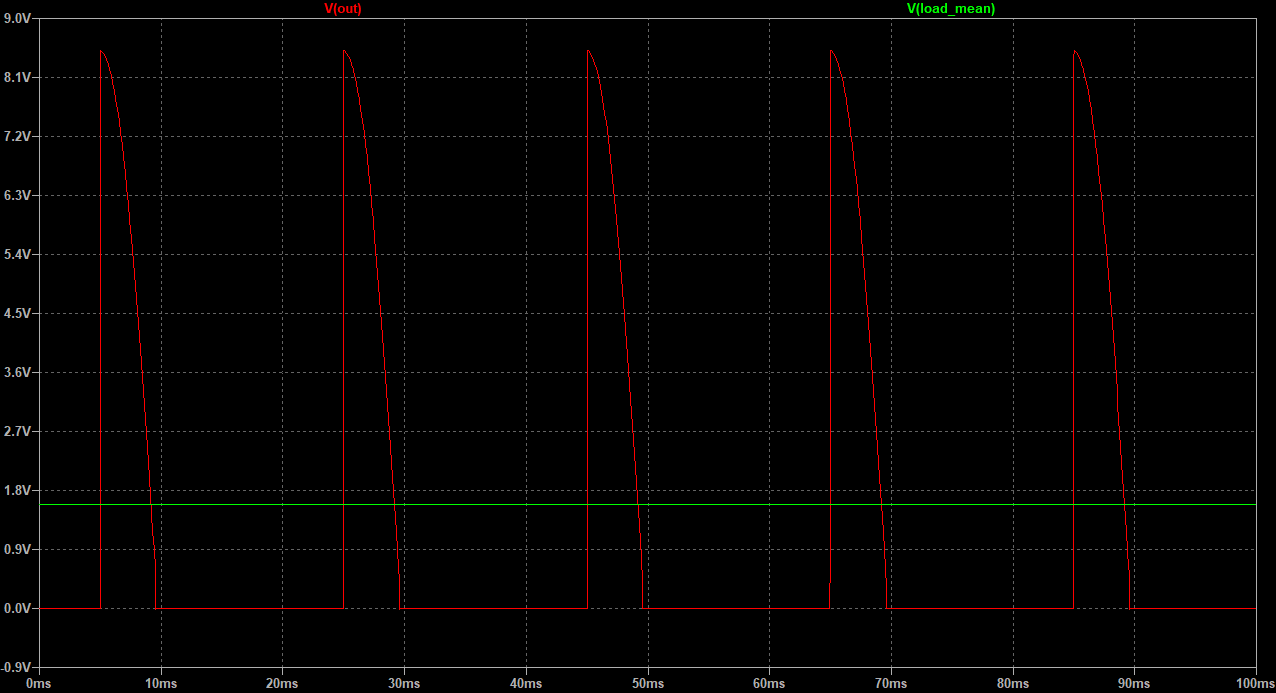
\includegraphics[width=\textwidth]{1_out_mean_v.png}
    \caption{Среднее значение напряжения на нагрузке.}
    \label{fig:1_out_mean_v}
\end{figure}

Сделаем 10 измерений среднего напряжения на нагрузке, изменяя угол включения от $0^\circ$ до $180^\circ$ и занесем полученные измерения и соответствующие им углы включения в таблицу:

\begin{center}
\begin{tabular}{ c|c c c c c c c c c c c } 
 $\alpha$ & $0^\circ$ & $18^\circ$ & $36^\circ$ & $54^\circ$ & $72^\circ$ & $90^\circ$ & $108^\circ$ & $126^\circ$ & $144^\circ$ & $162^\circ$ & $180^\circ$ \\ 
 \hline
 $V_{load_{mean}}$ & $3.18$ & $3.1$ & $2.88$ & $2.53$ & $2.08$ & $1.59$ & $1.1$ & $0.66$ & $0.30$ & $0.07$ & $0$ \\ 
\end{tabular}
\end{center}

\begin{figure}[H]
    \centering
    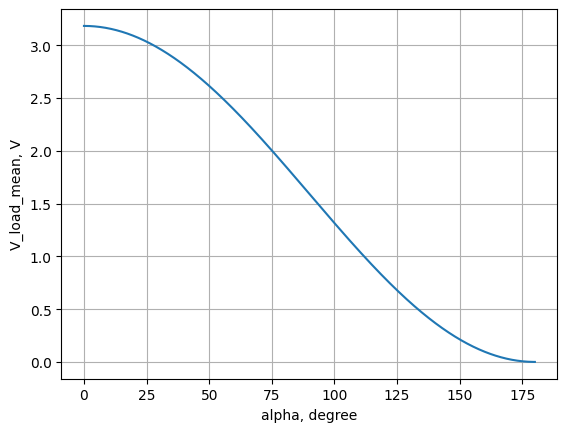
\includegraphics[width=0.7\textwidth]{v_load_mean_degree.png}
    \caption{Регулировочная характеристика управляемого выпрямителя.}
    \label{fig:v_load_mean_degree}
\end{figure}

\subsubsection*{Исследование работы тиристорного регулятора мощности}
Реализуем схему тиристорного регулятора мощности:
\begin{figure}[H]
    \centering
    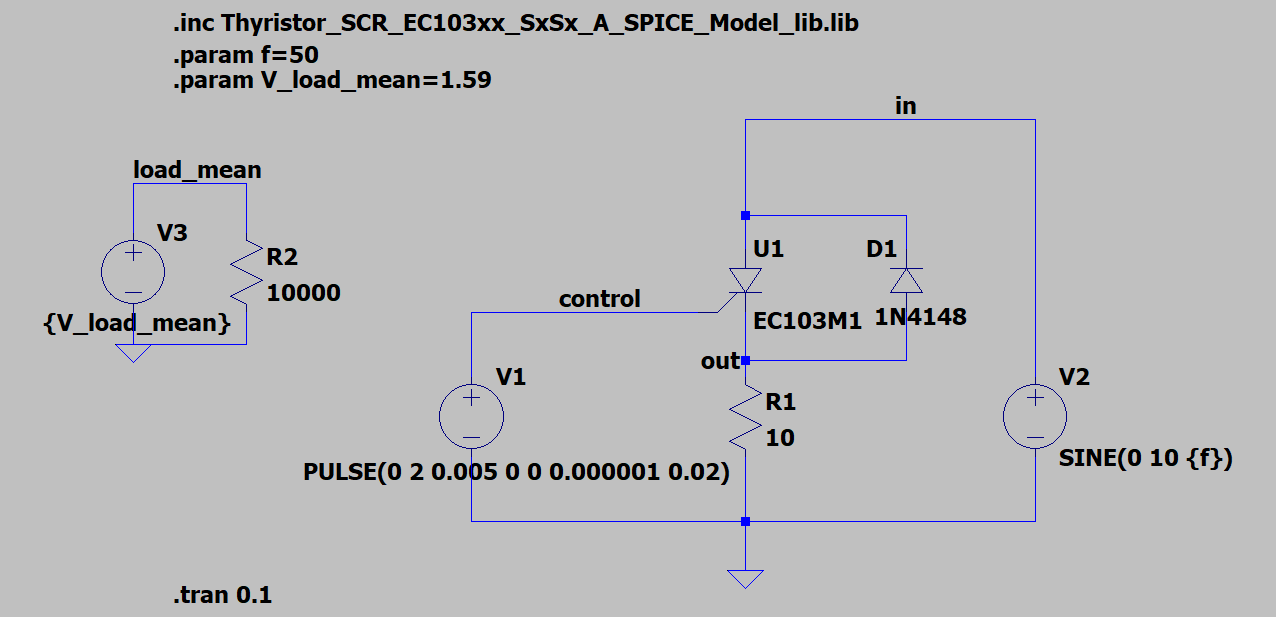
\includegraphics[width=0.7\textwidth]{2_scheme.png}
    \caption{Схема моделирования тиристорного регулятора мощности.}
    \label{fig:2_scheme}
\end{figure}

Настройки источников входного и управляющего напряжения оставим такими же как и в предыдущем пункте работы. \\
\begin{figure}[H]
    \centering
    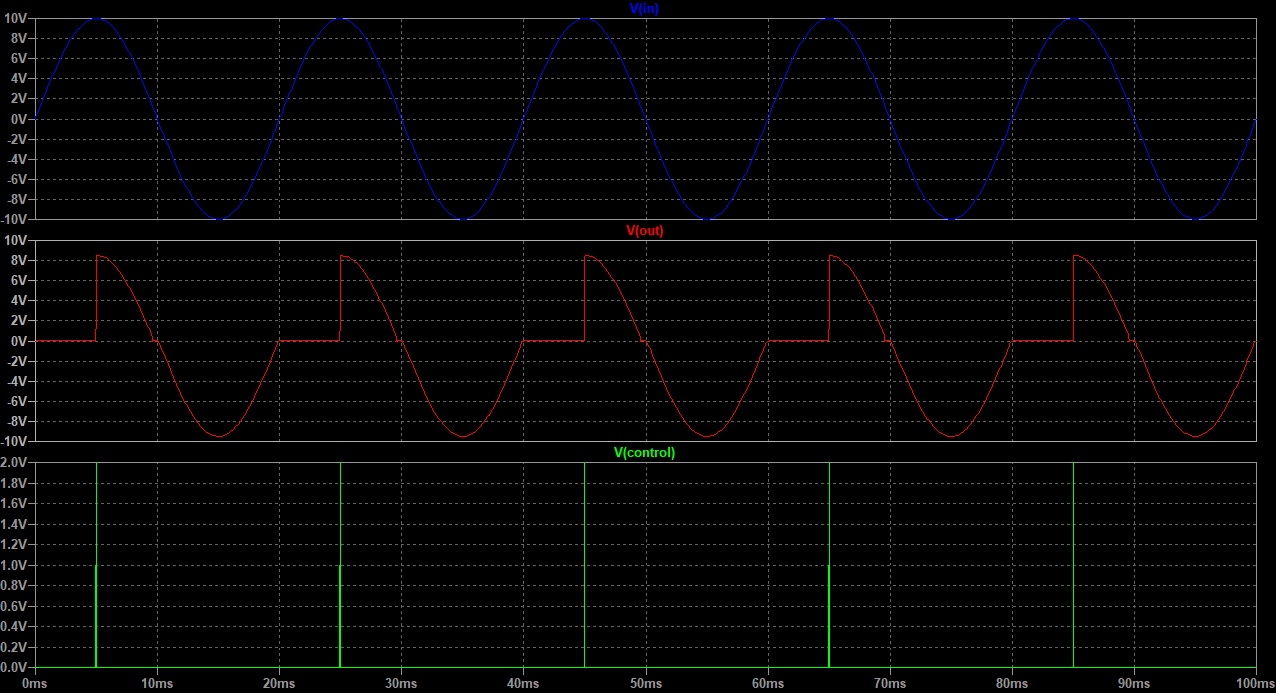
\includegraphics[width=\textwidth]{2_out_in_control_v.png}
    \caption{Осциллограммы входного, выходного и управляющего напряжений.}
    \label{fig:2_out_in_control_v}
\end{figure}

Вычислим действующее напряжение на выходе регулятора:
\[
    V_{eff} = \sqrt{\frac{1}{2\pi} \int_{\alpha}^{2\pi} V_{in}^2 \,d(\omega t)} = V_{{in}_{amp}} \sqrt{\frac{1}{8\pi}(4\pi - 2\alpha + \sin{2\alpha})} = | \ \alpha=90^\circ=\frac{\pi}{2}, \ V{{in}_{amp}} = 10 \ V \ | = 6.12 \ V.
\]

Отобразим действующее значение напряжения на нагрузке на графике:
\begin{figure}[H]
    \centering
    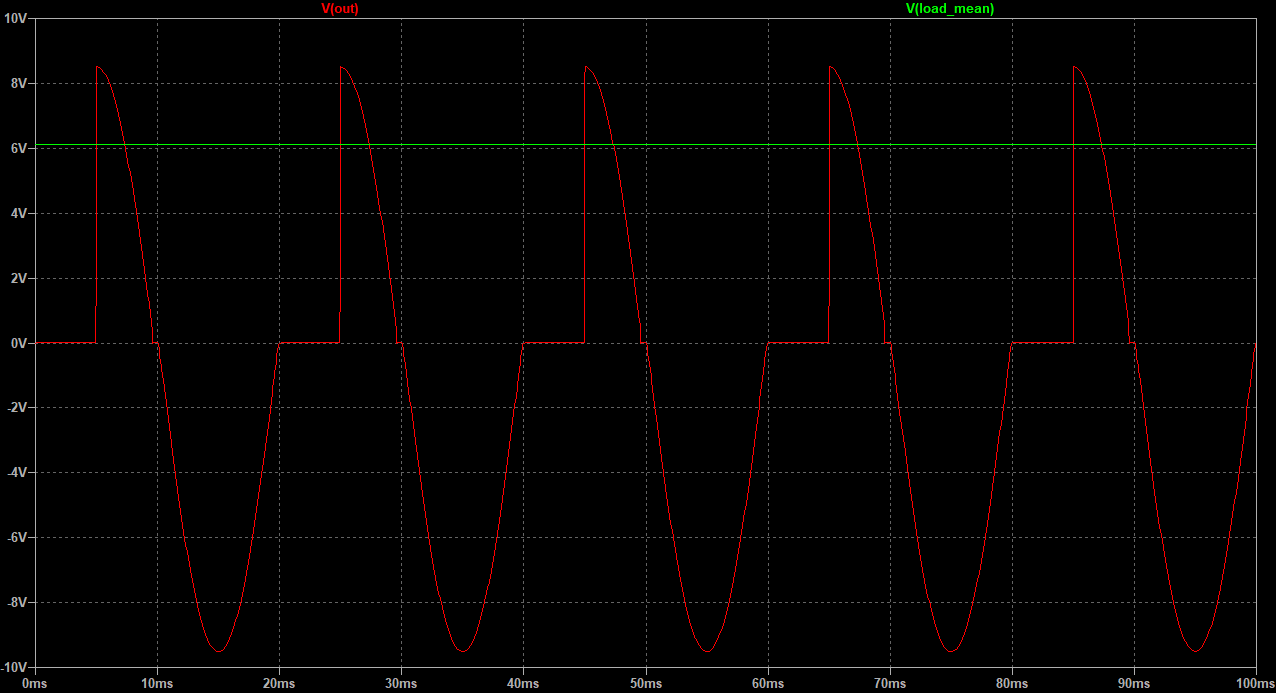
\includegraphics[width=\textwidth]{2_out_mean_v.png}
    \caption{Действующее значение напряжения на нагрузке.}
    \label{fig:2_out_mean_v}
\end{figure}

Сделаем 10 измерений действующего напряжения на нагрузке, изменяя угол включения от $0^\circ$ до $180^\circ$ и занесем полученные измерения и соответствующие им углы включения в таблицу:

\begin{center}
\begin{tabular}{ c|c c c c c c c c c c c } 
 $\alpha$ & $0^\circ$ & $18^\circ$ & $36^\circ$ & $54^\circ$ & $72^\circ$ & $90^\circ$ & $108^\circ$ & $126^\circ$ & $144^\circ$ & $162^\circ$ & $180^\circ$ \\ 
 \hline
 $V_{eff}$ & $7.07$ & $7.06$ & $6.98$ & $6.8$ & $6.51$ & $6.12$ & $5.72$ & $5.36$ & $5.12$ & $5.02$ & $5$ \\ 
\end{tabular}
\end{center}

\begin{figure}[H]
    \centering
    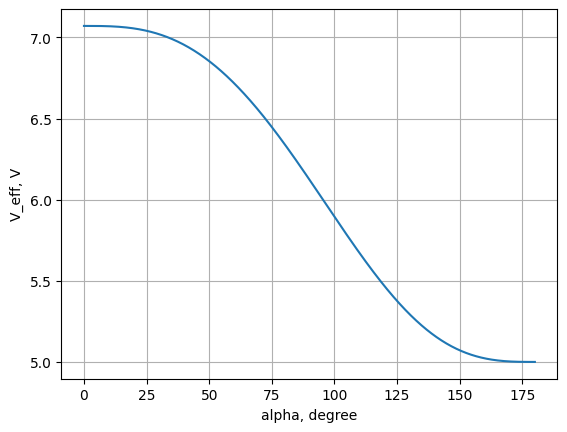
\includegraphics[width=0.7\textwidth]{v_eff_degree.png}
    \caption{Регулировочная характеристика регулятора мощности.}
    \label{fig:v_eff_degree}
\end{figure}

\section*{Выводы}
В данной лабораторной работе были исследованы тиристоры - полупроводниковые прибор, выполненные на основе монокристалла полупроводника с тремя или более p-n-переходами и имеющие два устойчивых состояния: низкой и высокой проводимости. \\
Мы рассматривали вид тиристора - тринистор - прибор с тремя электрическими выводами — анодом, катодом и управляющим электродом. \\
\ \\
В первой части работы был смоделирован управляемый однополупериодный выпрямитель на основе тринистора. За счет изменения входного сигнала можно изменять \emph{угол включения} прибора, который определяем момент включения тринистора. \\
\ \\
Во второй части был исследован регулятор мощности, состоящий из последовательно соединенных с сопротивлением нагрузки встречно-параллельного тиристора и выпрямительного диода. Регулирование мощности, выделяемой на нагрузке, осуществляется за счет изменения угла включения тиристора с помощью управляющих импульсов, поступающих со схемы управления. \\
Особенностью рассмотренной схемы является то, что регулирование производится только в течение положительного полупериода входного напряжения. Поэтому мощность в нагрузке будет изменяться в диапазоне $[50\%, 100\%]$ от
максимального значения.

\end{document}